\documentclass{article}

% Math formulas
\usepackage{amsmath}

\usepackage{minted}


% Zeichenkodierung und Schriftart
\usepackage[utf8]{inputenc}
\usepackage[T1]{fontenc}
\usepackage{lmodern}

% TikZ
\usepackage{tikz}
\tikzset{
  level/.style={
    sibling distance=30mm/#1
  },
  level distance=10mm,
}

 \tikzset{
  every node/.style={
    draw,
    circle,
    inner sep=0pt,
    minimum width=15pt
  },
  thick
}


\begin{document}
\title{Dynamic Programming}
\author{Juan Andrés Osorio Escobar}
\date{\today}
\maketitle


\begin{abstract}
Dynamic Programming (short \textbf{\emph{DP}}) refers to a problem solving paradigm,
  which seeks to solve a problem by solving related subproblems and combining their solutions to solve the main problem.
  As these subproblems may be encountered repeatedly along the solving process, DP algorithms store their solution, so 
  that the same computation is never done twice, potentially making the computation for the main solution much faster at 
  the cost of increased memory usage. DP is often applied to solve optimization problems and counting problems.

  In order for a problem to be applicable to optimization it must exhibit the following traits:

  \begin{itemize}
    \item \textbf{Optimal substructures}: The solution for a subproblem is part of the solution of the original problem \cite{halim2013competitive}.
    \item \textbf{Ovelapping subproblems}: When a recursive algorithm repeatedly revisist the same subproblem in different branches along its recursion tree, we say that the problem has overlapping subproblems \cite{cormen2009introduction}. This is the key characteristic
    which allows the search space for a problem to be drastically reduced \cite{halim2013competitive}.
  \end{itemize}
  
  When these DP criteria are met, DP solutions may reduce the run time of a problem from exponential 
  time complexity (using complete search algorithms), to polynomial time complexity. DP algorithms can be implemented
  in one of two ways: either recursively/top-down with memoization, or bottom-up. Both methods make use of a table in which the solution to subproblems are stored.
  We shall revisit also both techniques and analyze their pros and cons.

  
  
\bibliographystyle{acm}
\bibliography{references.bib}
  
\end{abstract}

\tableofcontents

 
 \section{introduction}


What is dynamic programming? it really sounds like one of those big buzzwords that seem to
attract big audiences that tend to follow trends. But put in simple words, Dynamic Programming is just a tabular method, 
which reduces a lot of duplicate computations on a problem.How does dynamic programming work? lets have a look at an example first: The fibonacci numbers,
which form a sequence defined as follows:

  \[
    fib(n) = \left\{\begin{array}{lr}
      n, & \text{for } n = 1, n = 2\\
      fib(n-1) + fib(n-2), & \text{otherwise}
      \end{array}\right\}
  \]

we could write a simple program to compute the nth fibonacci number as follows:

\begin{minted}[mathescape, linenos]{python}

def fibonacci(n):
  if (n <= 1):
    return n
  else :
    return fibonacci(n - 1) + fibonacci(n + 2)

\end{minted}


to get a rough picture of the space complexity for this program, we could depict the steps
the program would take to compute an arbitrary number n, in the form of a tree. For n = 6, we have:


\begin{figure}[ht]
  \centering
  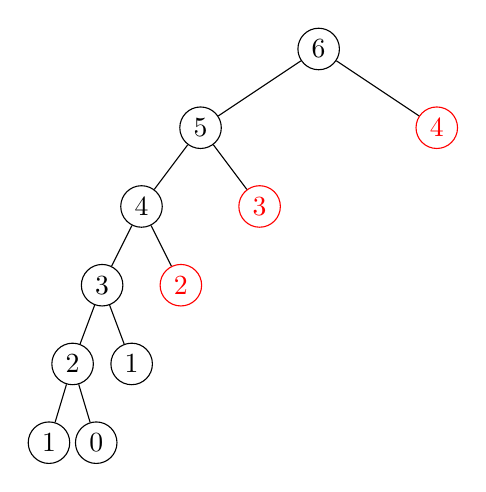
\begin{tikzpicture}
    \node {6}
      child { node {5}
        child { node {4} 
          child{ node {3} 
            child { node {2}
              child {node {1}}
              child {node {0}}
            }
            child { node {1}}
          }
          child{ node[color=red] {2} }
        }
        child { node[color=red] {3} }
      }
      child { node[color=red] {4}
      };
  \end{tikzpicture}
  \caption{Fibonacci recursion tree with $n = 6$}
  \label{fig:fib1}
\end{figure}

There are 6 levels in this call tree and although the red nodes in \autoref{fig:fib1} are 
not expanded, the algorithm has still to do all the work and visit this nodes until it gets to a node
labeled with one or with zero. We can easily see how this can get out of hands with higher numbers, the 
number of nodes is $O(2^n)$


\end{document}